\documentclass[../../main.tex]{subfiles}

\begin{document}

\section{Introduction}

In this chapter, we extend the 1D experiments to 2D. We will use the same datasets as the 1D experiments, but extend them to 2D and see how the models perform with the additional complexity. We will investigate the performance of the TETNP with a modified variant of the relative attention scheme we introduced in \autoref{sec:tetnp}. Finally, we will investigate the memory usage of the ConvNP and TETNP in 2D and compare it to the 1D case.

\section{Datasets}

We will use the same datasets as the 1D experiments, but extend them to 2D. From both datasets, choose to sample $N_c = 64$ context points and $N_t = 128$ target points. The context and target region for the sawtooth dataset defined as $x_1, x_2 \in [-2, 2]$ and $x_1, x_2 \in [-4, 4]$ respectively. For the Gaussian Process dataset, the context and target region are defined as $x_1, x_2 \in [-4, 4]$ and $x_1, x_2 \in [-8, 8]$ respectively.  

In our plots, the context region will be inside a black dotted box and the target region will be inside a red dotted box. The extrapolation region is outside the target region.

\subsection{Gaussian Process}

The 2D Gaussian Process is the natural extension of the 1D Gaussian Process described in \autoref{sec:1d-gp-dataset} where we use the squared exponential kernel. We continue to use the same range of lengthscale across both input dimensions as the 1D Gaussian Process. 

% The following plots show some samples from the GP dataset.

% \todo{Add plots of GP dataset}


\subsection{Sawtooth}

The 2D Sawtooth dataset is the natural extension of the 1D Sawtooth dataset described in \autoref{sec:1d-sawtooth-dataset}. We continue to use the same frequency $f$ and noise $n$ across both input dimensions as the 1D Sawtooth dataset.

% The following plots show some samples from the Sawtooth dataset.

% \todo{Add plots of Sawtooth dataset}

\subsection{Restricted Sawtooth}

The restricted sawtooth limits the `direction of travel' of the sawtooth function to the line of $x_1 = x_2$ or $x_1 = -x_2$. Under this dataset the model only learn a subset of the `full sawtooth' function. We can use this probe how well the models can generalize to samples from the full sawtooth function.

% The following plots show some samples from the Restricted Sawtooth dataset.

\section{Post or Pre MLP}

In our original formulation of the TETNP (\autoref{sec:tetnp}) we pass the matrix of differences ($\bm{\Delta}$) between $x$ values through an MLP to apply non-linearities then add it to the dot product attention \autoref{eq:relative-attention}, whilst this performs well we can also consider applying this non-linearity after combining the dot product attention and the relative attention, this method is called the `Post MLP'. The formulation of the `Post MLP' is as follows:

\begin{align}
	\text{Attention}(\bm{Q}, \bm{K}, \bm{V}, \bm{X}) &= \text{softmax}\left(\bm{E} \right) \bm{V}
\end{align}
\begin{align}
	\text{Pre MLP:} \quad \bm{E_{ij}} &= \bm{D_{ij}}+ \text{MLP}(\bm{\Delta_{ij}})\\
    \text{Post MLP:} \quad \bm{E_{ij}} &= \text{MLP}(\texttt{cat}[ \bm{D_{ij}}, \bm{\Delta_{ij}}])
\end{align}
Where 
\begin{align}
     \bm{D_{ij}} = \bm{q_i} \cdot \bm{k_j}  /\sqrt{d_k} \quad \quad    \bm{\Delta_{ij}} = \bm{x_i} - \bm{x_j}
\end{align}


We will investigate the performance of the TETNP with the `Post MLP' compared to the original `Pre MLP'. The Sawtooth dataset is chosen for this experiment as it is more difficult to learn than the Gaussian Process dataset, thereby allowing us to observe the differences between the two functions more clearly.

% Figure ./post-pre-kernel.pdf
\begin{figure}[H]
    \centering
    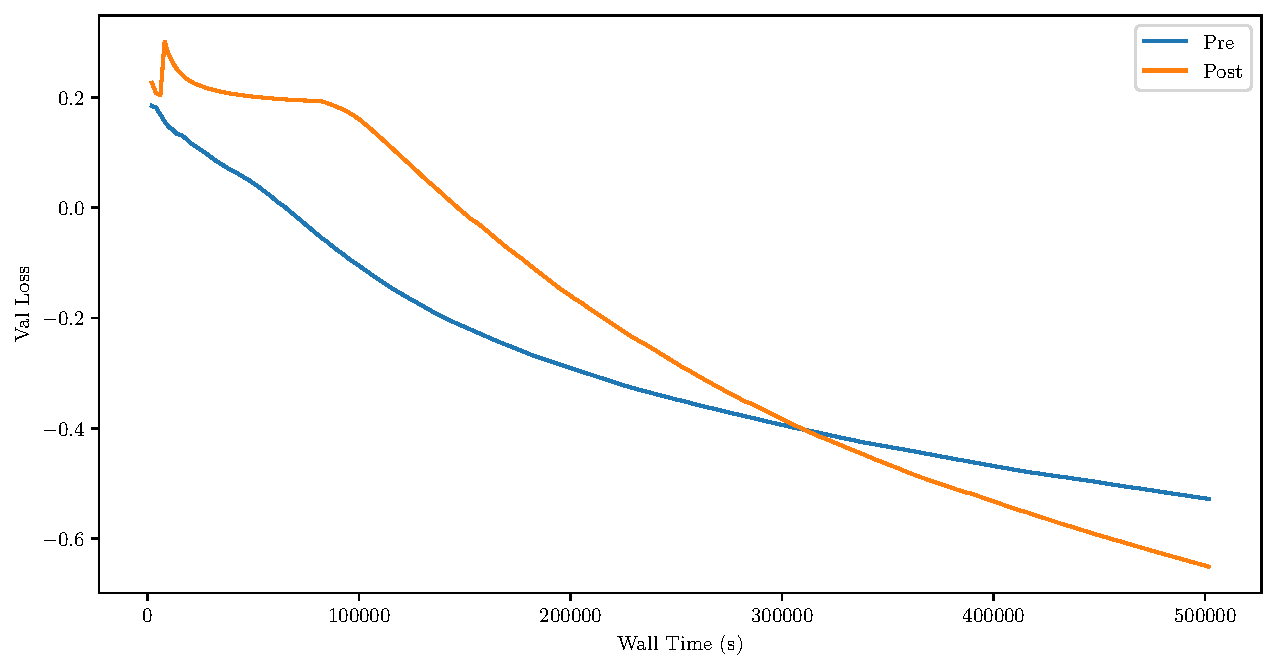
\includegraphics[width=0.6\linewidth]{./fig/post-pre-kernel.pdf}
    \caption{Validation Loss of TETNP with the `Post MLP' and `Pre MLP' on the 2D Sawtooth Dataset. Lower validation loss is better.}
    \label{fig:post-pre-kernel}
\end{figure}


The results show that the TETNP with the `Post MLP' outperforms the TETNP with the `Pre MLP' by quite a large margin. Trivially the Post function can further refine the dot product attention through the MLP whilst in the `Pre' function the MLP is \emph{only} applied to the $\bm{\Delta}$ matrix. The computational complexity of these two functions are not too different as the MLP are small and applied to matrices of the same size.

\section{Model Comparison}

We have discovered in the 1D section that the TETNP outperforms the vanilla TNP in all cases, hence for the 2D experiments we will only compare the ConvNP to the TETNP. When performing our experiments we will use models which are both 1 million parameters in size, to ensure a fair comparison. The technical details of the ConvNP and TETNP are described in \autoref{sec:convnp-2d-appendix} and \autoref{sec:tnp-appendix} respectively.

\subsection{Gaussian Process}

As mentioned previously, the Gaussian Process dataset is not very difficult to learn and the ConvNP and TETNP both perform very well on this dataset with the TETNP outperforming the ConvNP by a small margin as shown in \autoref{tab:gp-2d-val-doss}.

\begin{table}[ht]
    \centering
    \begin{tabular}{lc}
        \toprule
        Model  & Validation Loss \\
        \midrule
        ConvNP & 1.168           \\
        TETNP  & 1.134           \\
        \bottomrule
    \end{tabular}
    \caption{Validation Loss of ConvNP and TETNP on the 2D Gaussian Process dataset after training for 4 hours using 1 million parameters models and 64 context points. Lower is better.}
    \label{tab:gp-2d-val-doss}
\end{table}

Observing the samples from the ConvNP and TETNP for the 2D Gaussian Process dataset \autoref{fig:high-freq-2d-gps}, we note that both models successfully  learn the underlying process, with the TETNP being able to perform slightly better than the ConvNP. Given the smooth nature of the GP dataset, it is not surprising that both models perform well. To highlight the differences between the ConvNP and TETNP, we will proceed to the Sawtooth dataset which is more difficult to learn.

% \begin{figure}[H]
% 	\centering
% 	\subfloat[ConvNP (top plot is the model prediction and bottom is the ground truth GP)]{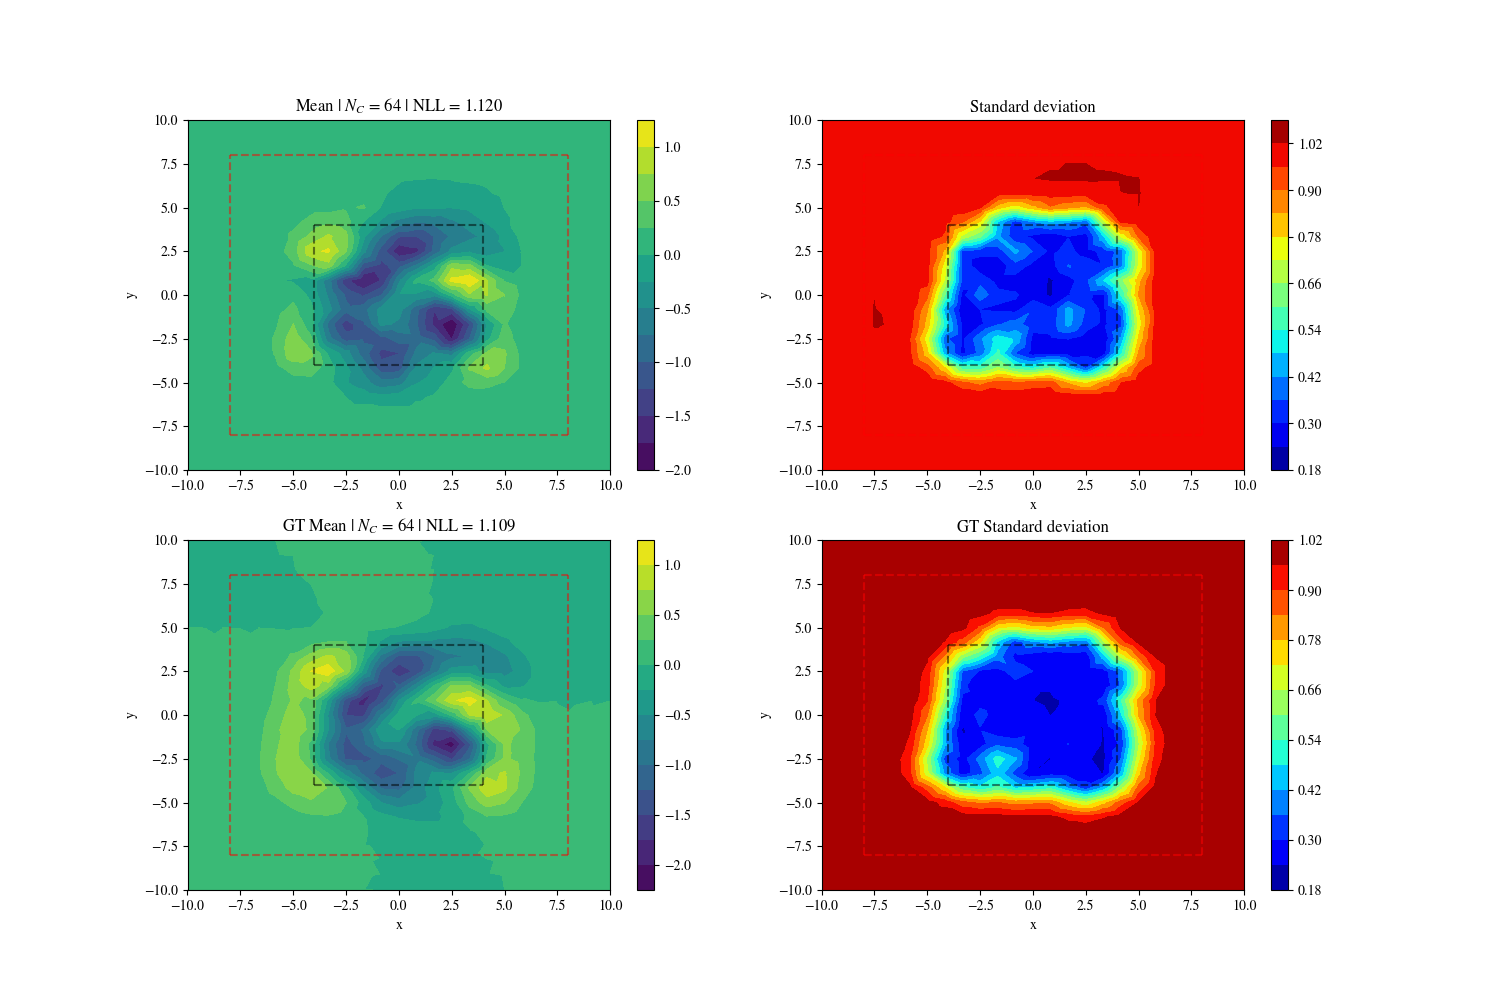
\includegraphics[width=0.8\linewidth]{./fig/gp/conv-gp-2d.png}}\\
% 	\subfloat[TETNP (top plot is the model prediction and bottom is the ground truth GP)]{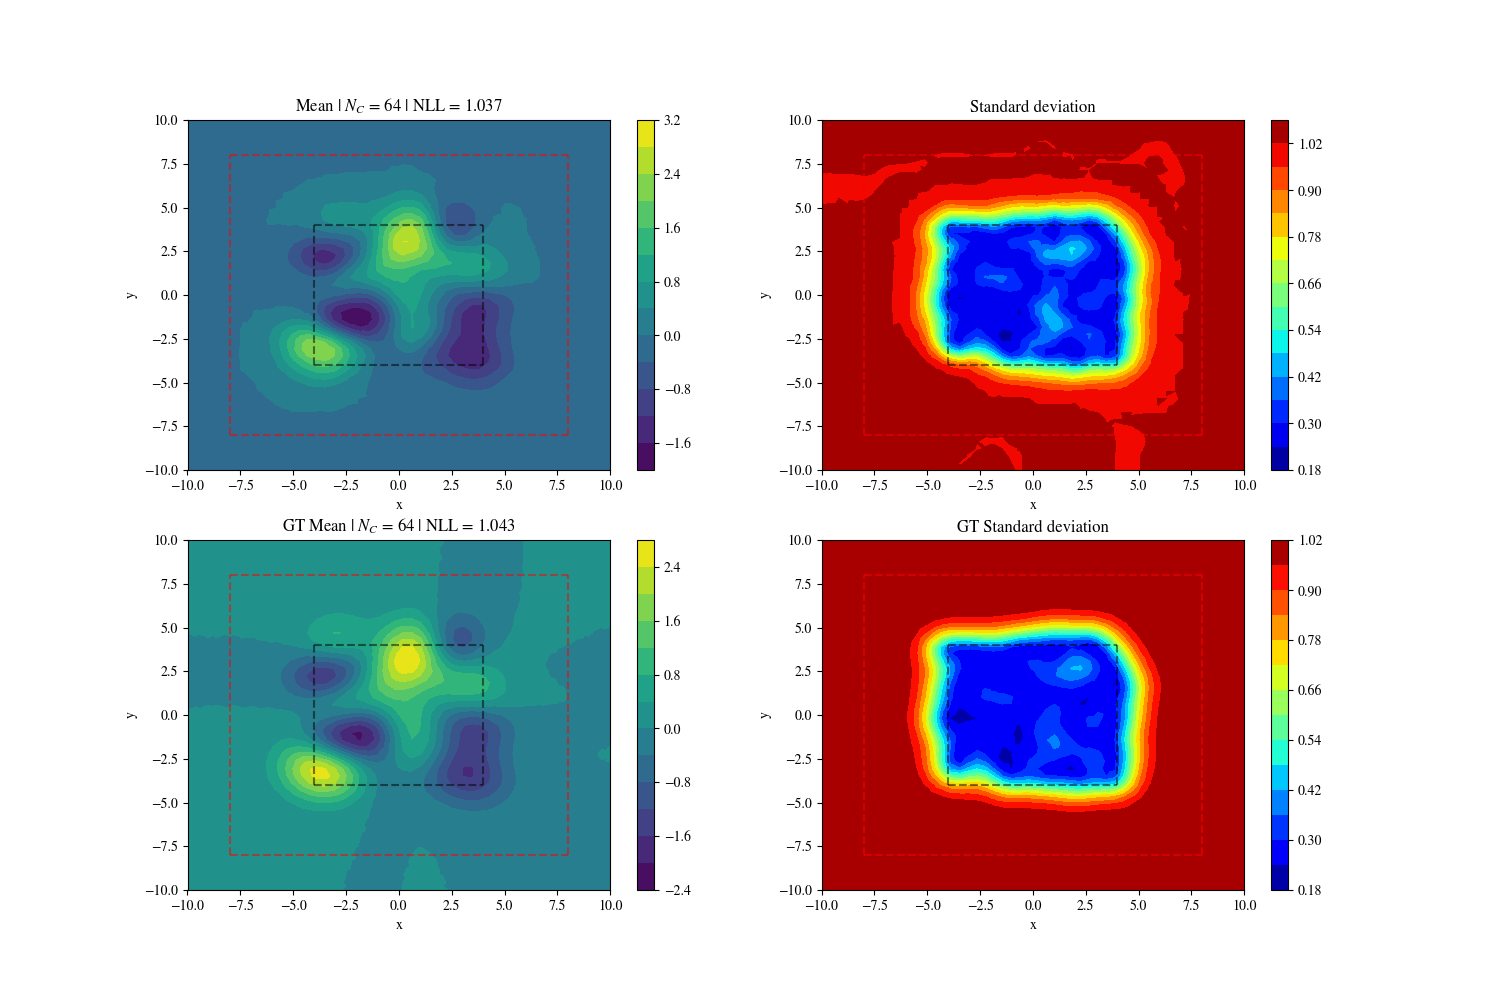
\includegraphics[width=0.8\linewidth]{./fig/gp/tetnp-gp-2d.png}}
% 	\caption{Samples from ConvNP and TETNP on a low frequency 2D Gaussian Process.}
% 	\label{fig:low-freq-2d-gps}
% \end{figure}

\begin{figure}[H]
	\centering
	\subfloat[ConvNP (top plot is the model prediction and bottom is the ground truth GP)]{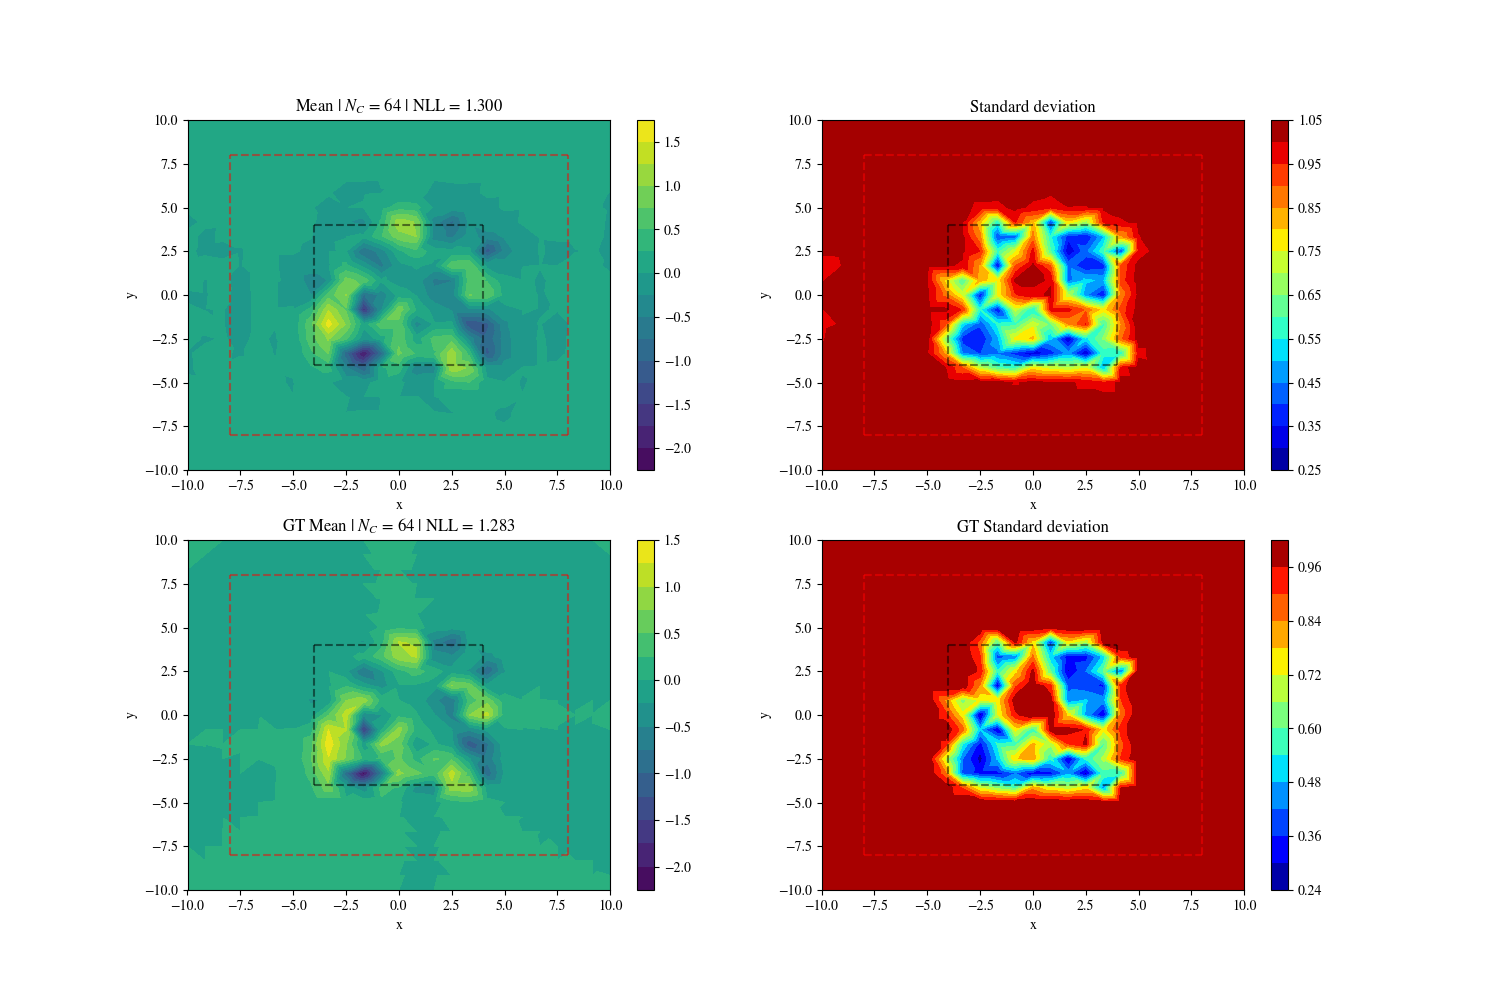
\includegraphics[width=0.8\linewidth]{./fig/gp/conv-gp-2d-2.png}}\\
	\subfloat[TETNP (top plot is the model prediction and bottom is the ground truth GP)]{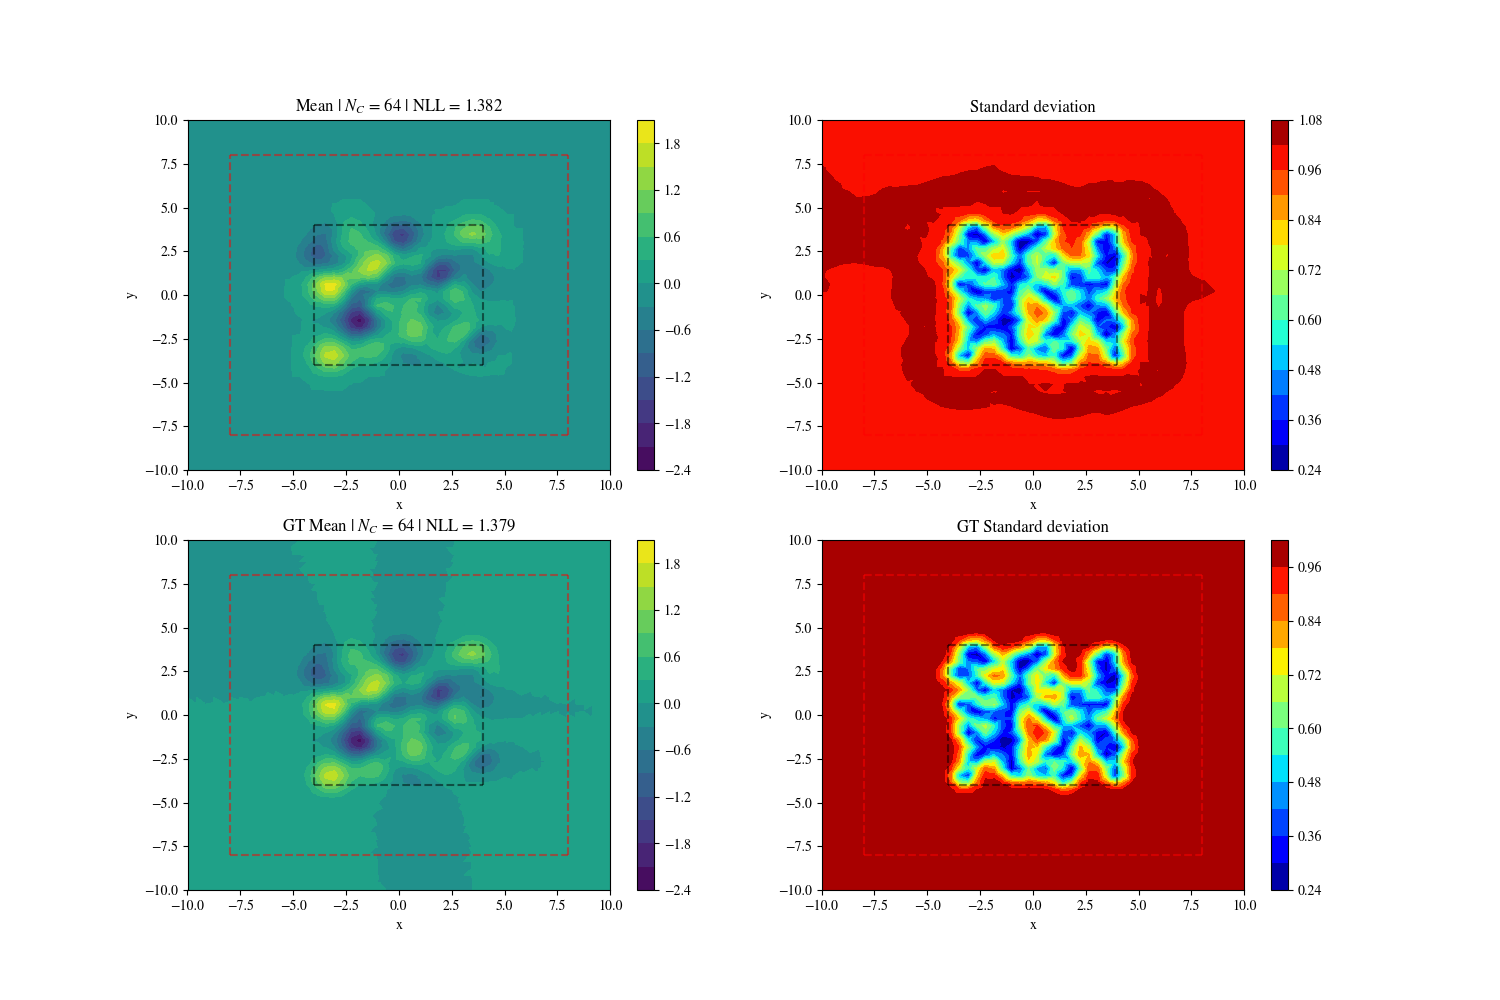
\includegraphics[width=0.8\linewidth]{./fig/gp/tetnp-gp-2d-2.png}}
	\caption{Samples from ConvNP and TETNP on a frequency 2D Gaussian Process using 64 context points.}
	\label{fig:high-freq-2d-gps}
\end{figure}

\subsection{Restricted Sawtooth and Rotational Equivariance}

As previously stated the restricted sawtooth dataset is a subset of the full sawtooth dataset which restricts the `direction of travel' of the sawtooth function to the line of $x_1 = x_2$ or $x_1 = -x_2$. Training the models on this dataset will highlight the generalization ability of the models.
% Figure ./fig/res-saw/te.png and ./fig/res-saw/conv.png

\begin{figure}[H]
    \centering
    \subfloat[TETNP]{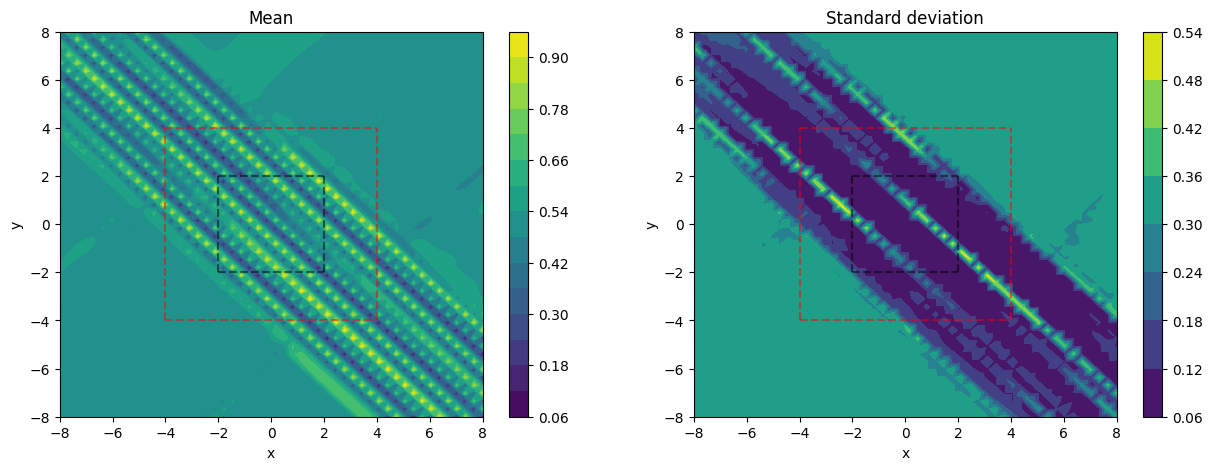
\includegraphics[width=0.8\linewidth]{./fig/res-saw/te.png}}\\
    \subfloat[ConvNP]{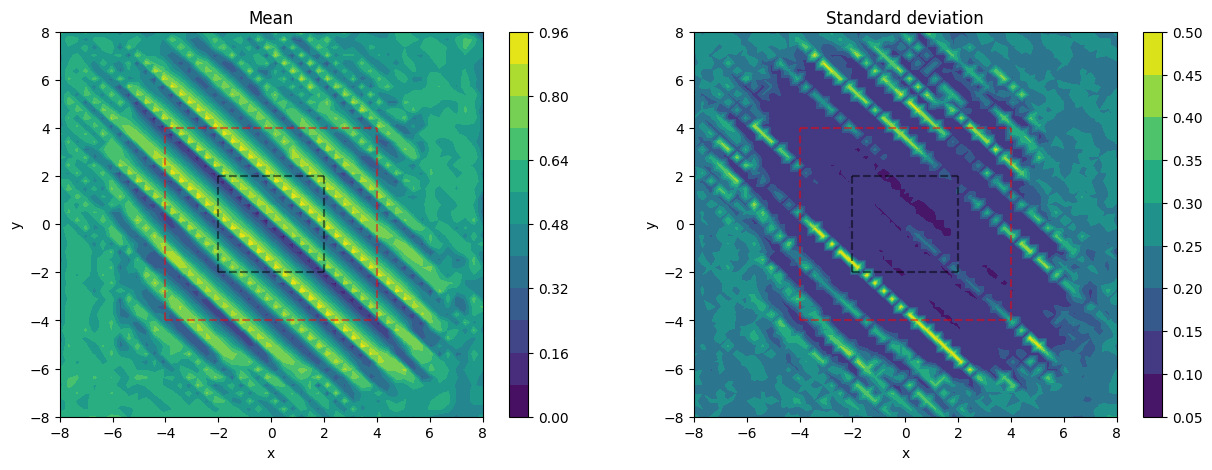
\includegraphics[width=0.8\linewidth]{./fig/res-saw/conv.png}}
    \caption{Samples from TETNP and ConvNP on the Restricted Sawtooth dataset. The region inside the black dotted box is the region the models were trained on and the region outside the black dotted box is the region the models were not trained on. 64 context points were used.}
    \label{fig:res-saw-preds}
\end{figure}

\autoref{fig:res-saw-preds} shows that the ConvNP performs excellently on this dataset, which is expected as CNNs use filters to learn features and patterns in the data explicitly, allowing them to perform excellently on extrapolation tasks (outside the black dotted box region). The TETNP on the other hand struggles to generalize fully within the target region (red dotted box) and outside the target region. Instead, it learns to extrapolate the sawtooth along one axis, but not the other. This brings to light a limitation of the Transformer architecture - it has very little interpretability which can result in unexpected behavior.

\emph{Is this TETNP able to generalize to the full sawtooth dataset?} To answer this question we apply the TETNP on a rotated version of the restricted sawtooth dataset which represents samples from the full sawtooth dataset.



% Figure ./fig/res-saw/no-re.png

\begin{figure}[H]
    \centering
    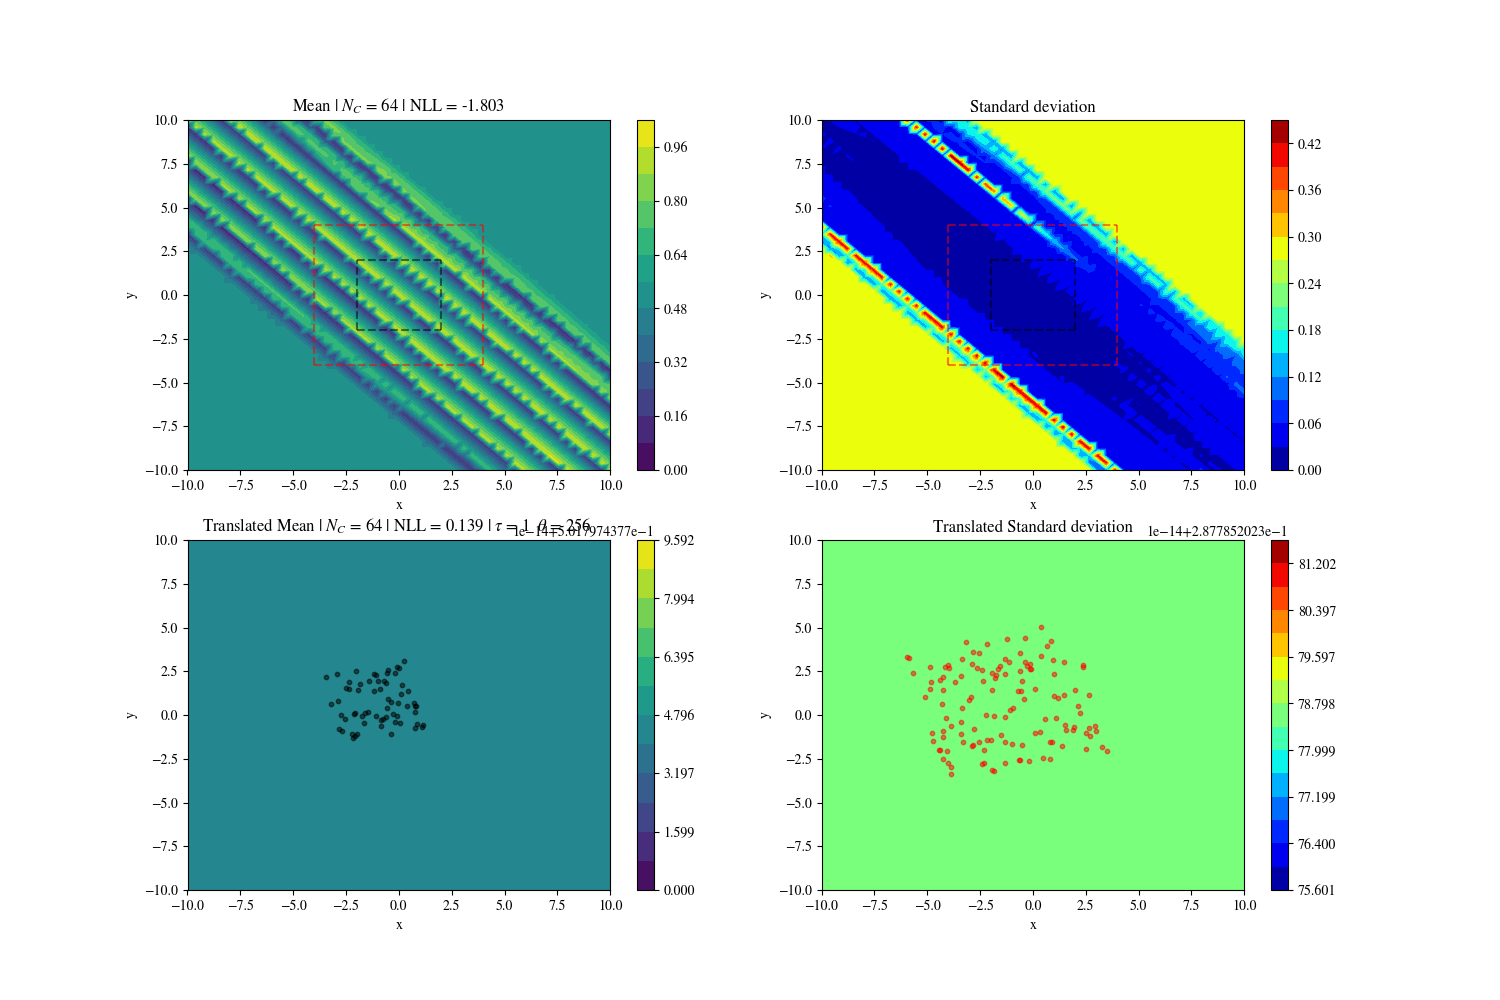
\includegraphics[width=1\linewidth]{./fig/res-saw/no-re.png}
    \caption{Generalization of the TETNP. The context points on the left are rotated by 45 degrees and  the inference is performed on this rotated set giving us the right plot.}
    \label{fig:no-re-saw-preds}
\end{figure}

In \autoref{fig:no-re-saw-preds}  illustrates the predictions when we rotate the context points by 45 degrees, clearly the TETNP completely fails, predicting only a constant mean and standard deviation. It struggles to generalize to rotations, which brings us to the question: \emph{Could introducing rotational equivariance to the TETNP help it generalize to the full sawtooth dataset?}

\subsubsection{Rotational Equivariance}

Introducing rotational equivariance (RE) is relatively straightforward. In our formulation of the Translation Equivariance Attention, we use a pairwise-difference matrix $\bm{\Delta}$ which contains the differences between the $\bm{x}$ values of all the data points.

\begin{align}
    \text{Not RE}: \quad &\bm{\Delta}_{ij} = \bm{x}_i - \bm{x}_j\\
    \text{RE}: \quad &\bm{\Delta}_{ij} = \|\bm{x}_i - \bm{x}_j\|_2
\end{align}

To introduce rotational equivariance we can simply take the L2 norm of the $\bm{\Delta}$ matrix which will give us the distance between all the data points. Distances are invariant to rotation, hence the TETNP should be rotationally equivariant. Using this new $\bm{\Delta}$ matrix we can train the TETNP on the restricted sawtooth dataset and observe if it can generalize to the full sawtooth dataset.

% Figure ./fig/res-saw/re.png

\begin{figure}[H]
    \centering
    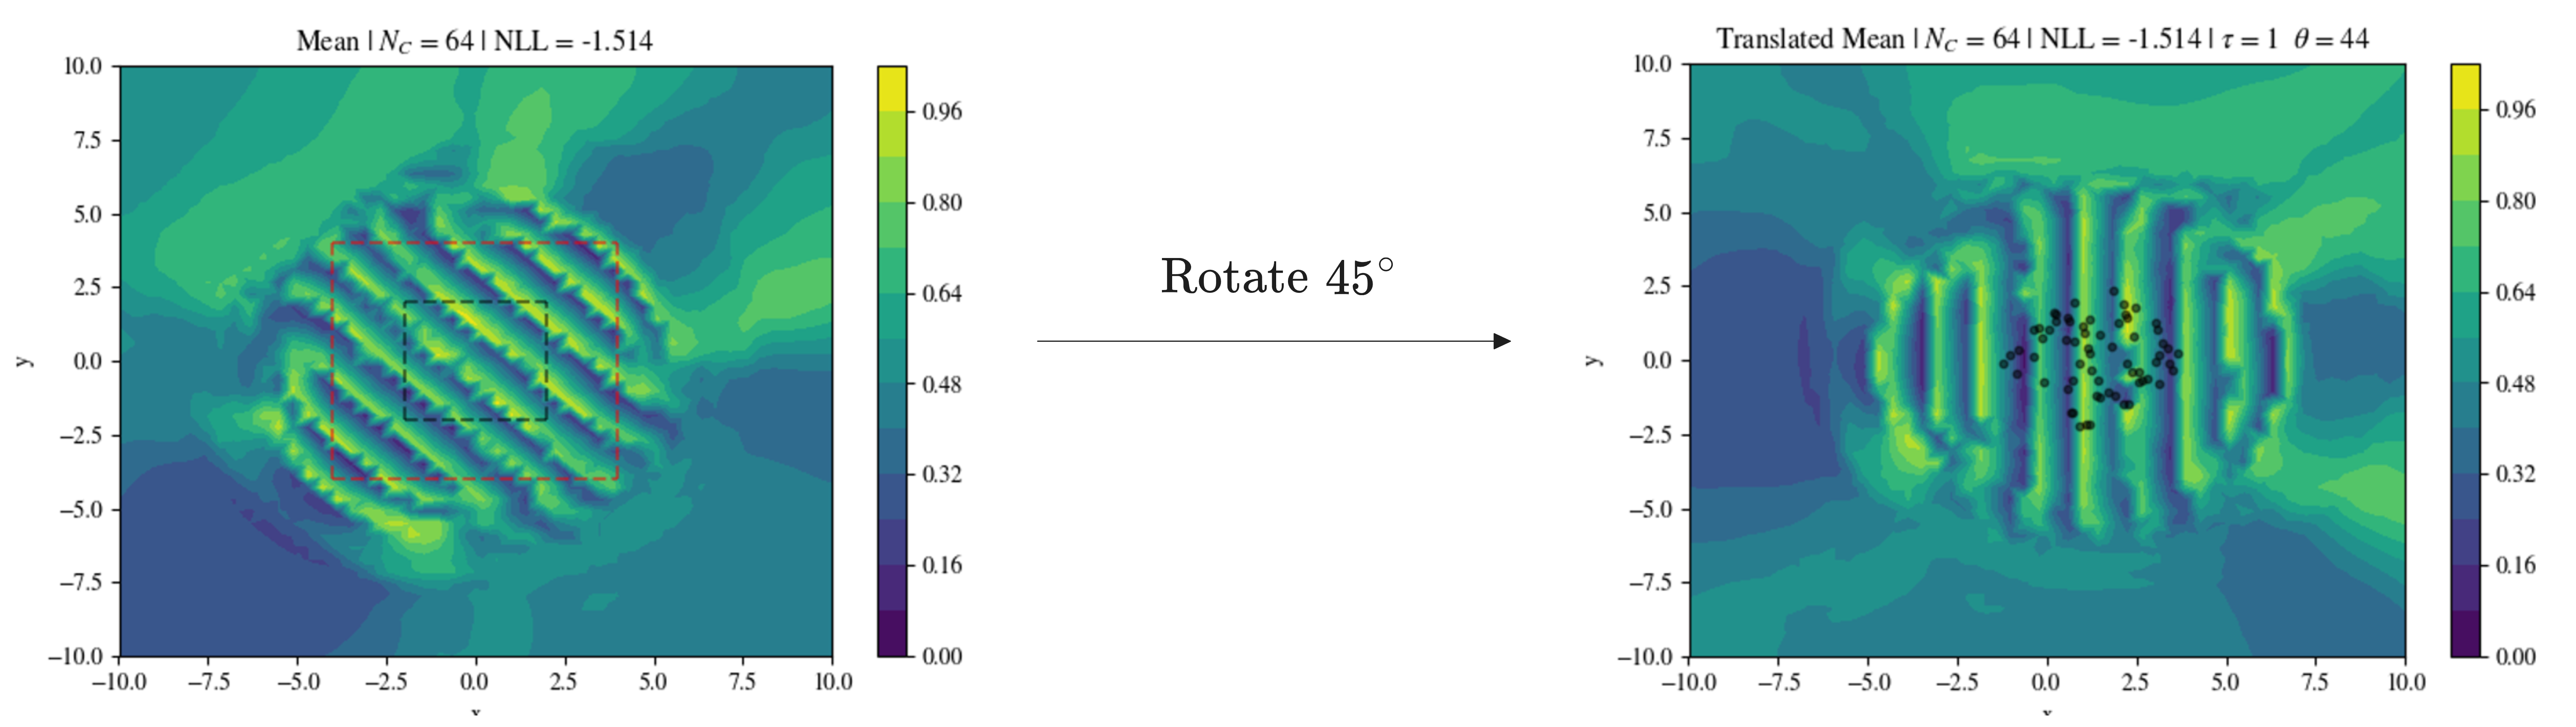
\includegraphics[width=1\linewidth]{./fig/res-saw/re.png}
    \caption{Generalization of the RE-TETNP. The context points on the left are rotated by 45 degrees and  the inference is performed on this rotated set giving us the right plot.}
    \label{fig:re-saw-preds}
\end{figure}

\autoref{fig:re-saw-preds} demonstrates a massive improvement in the TETNP's ability to generalize to the full sawtooth dataset. It has learned to extrapolate the sawtooth in all directions, which is a significant improvement over the non-RE TETNP. Hence, we can conclude that RE is beneficial for the case when the inherent structure of the data is rotationally invariant. This illustrates a massive benefit of the Transformer architecture, as \textbf{it is very easy to introduce inductive biases to the Transformer model}, which is not the case for CNNs.

However, as we will see in the next section, if the data given to the model contains samples from many directions, the model will learn to be RE.

\subsection{Full Sawtooth}

The full sawtooth dataset is the sawtooth function which is not restricted to any direction of travel. We observe that the TETNP is able to generalize to the full sawtooth dataset without the need for rotational equivariance \autoref{fig:full-saw-preds}. 

% Figure ./fig/saw/tetnp.png and ./fig/saw/tetnp2.png and ./fig/saw/tetnp3.png

\begin{figure}[H]
    \centering
    \subfloat[TETNP Sample 1]{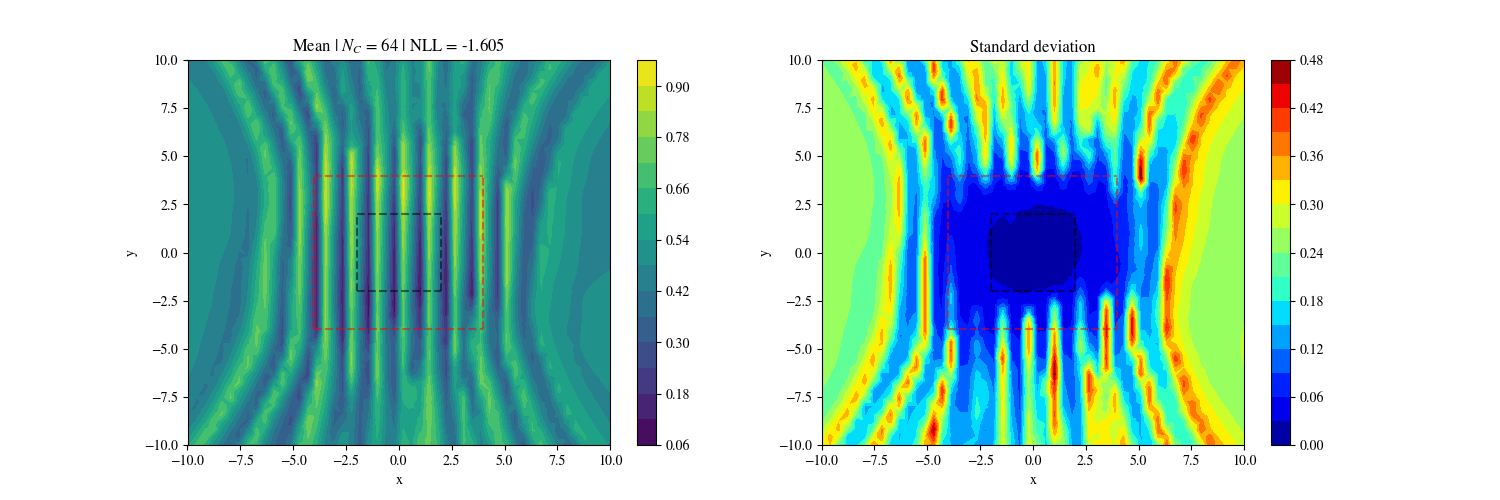
\includegraphics[width=0.3\linewidth]{./fig/saw/tetnp.png}}
    \subfloat[TETNP Sample 2]{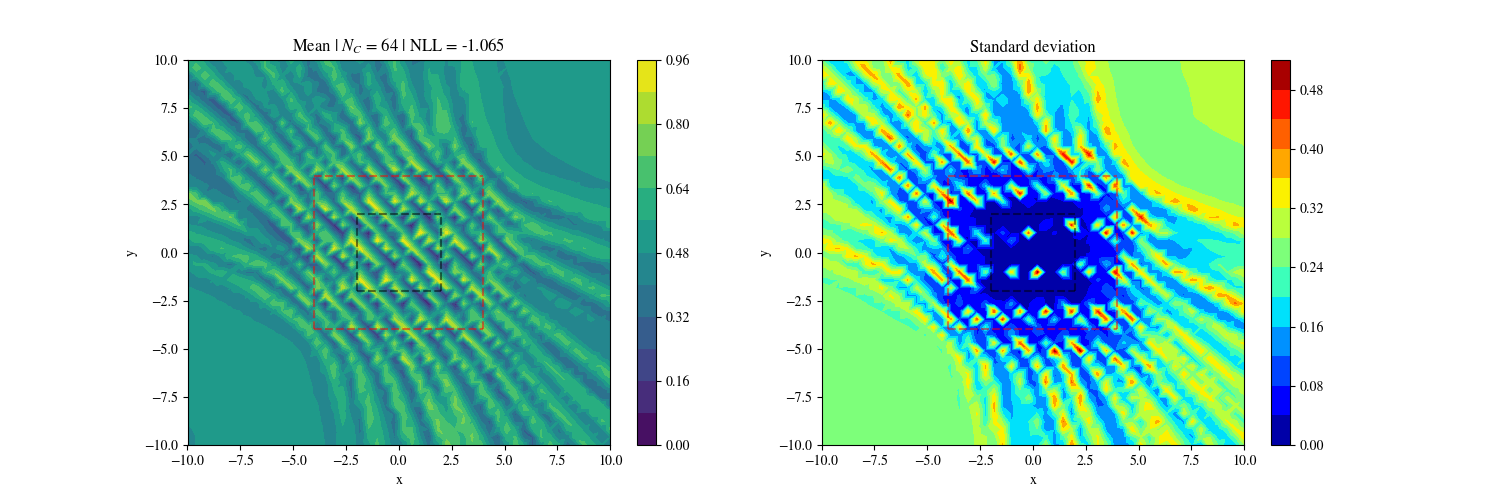
\includegraphics[width=0.3\linewidth]{./fig/saw/tetnp-2.png}}
    \subfloat[TETNP Sample 3]{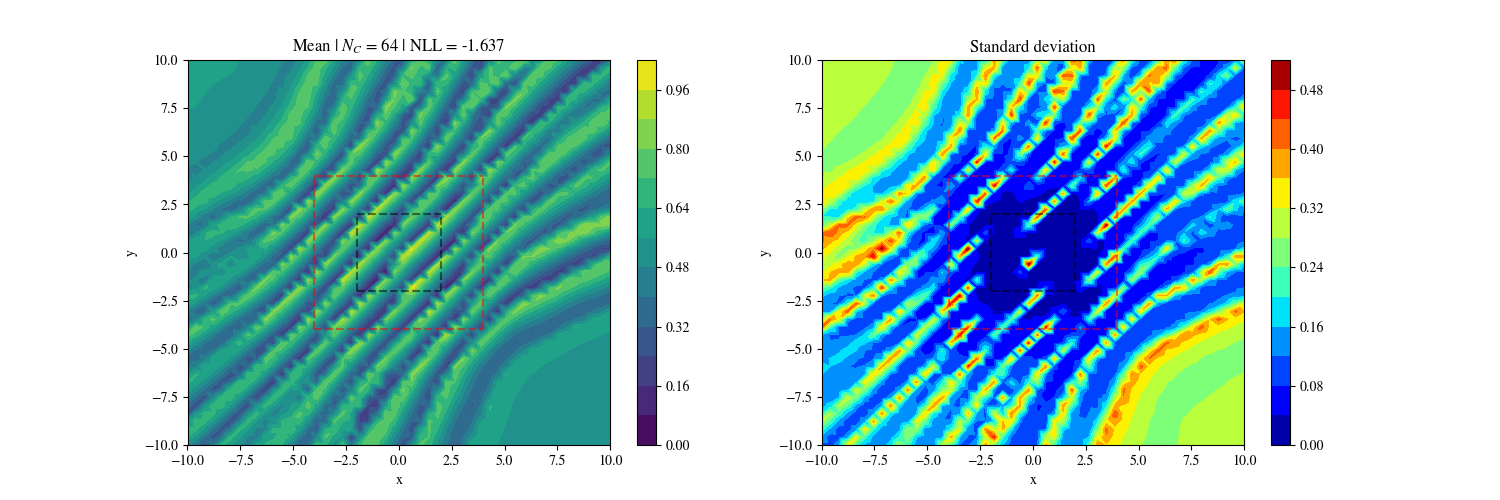
\includegraphics[width=0.3\linewidth]{./fig/saw/tetnp-3.png}}\\
    \subfloat[ConvNP Sample 1]{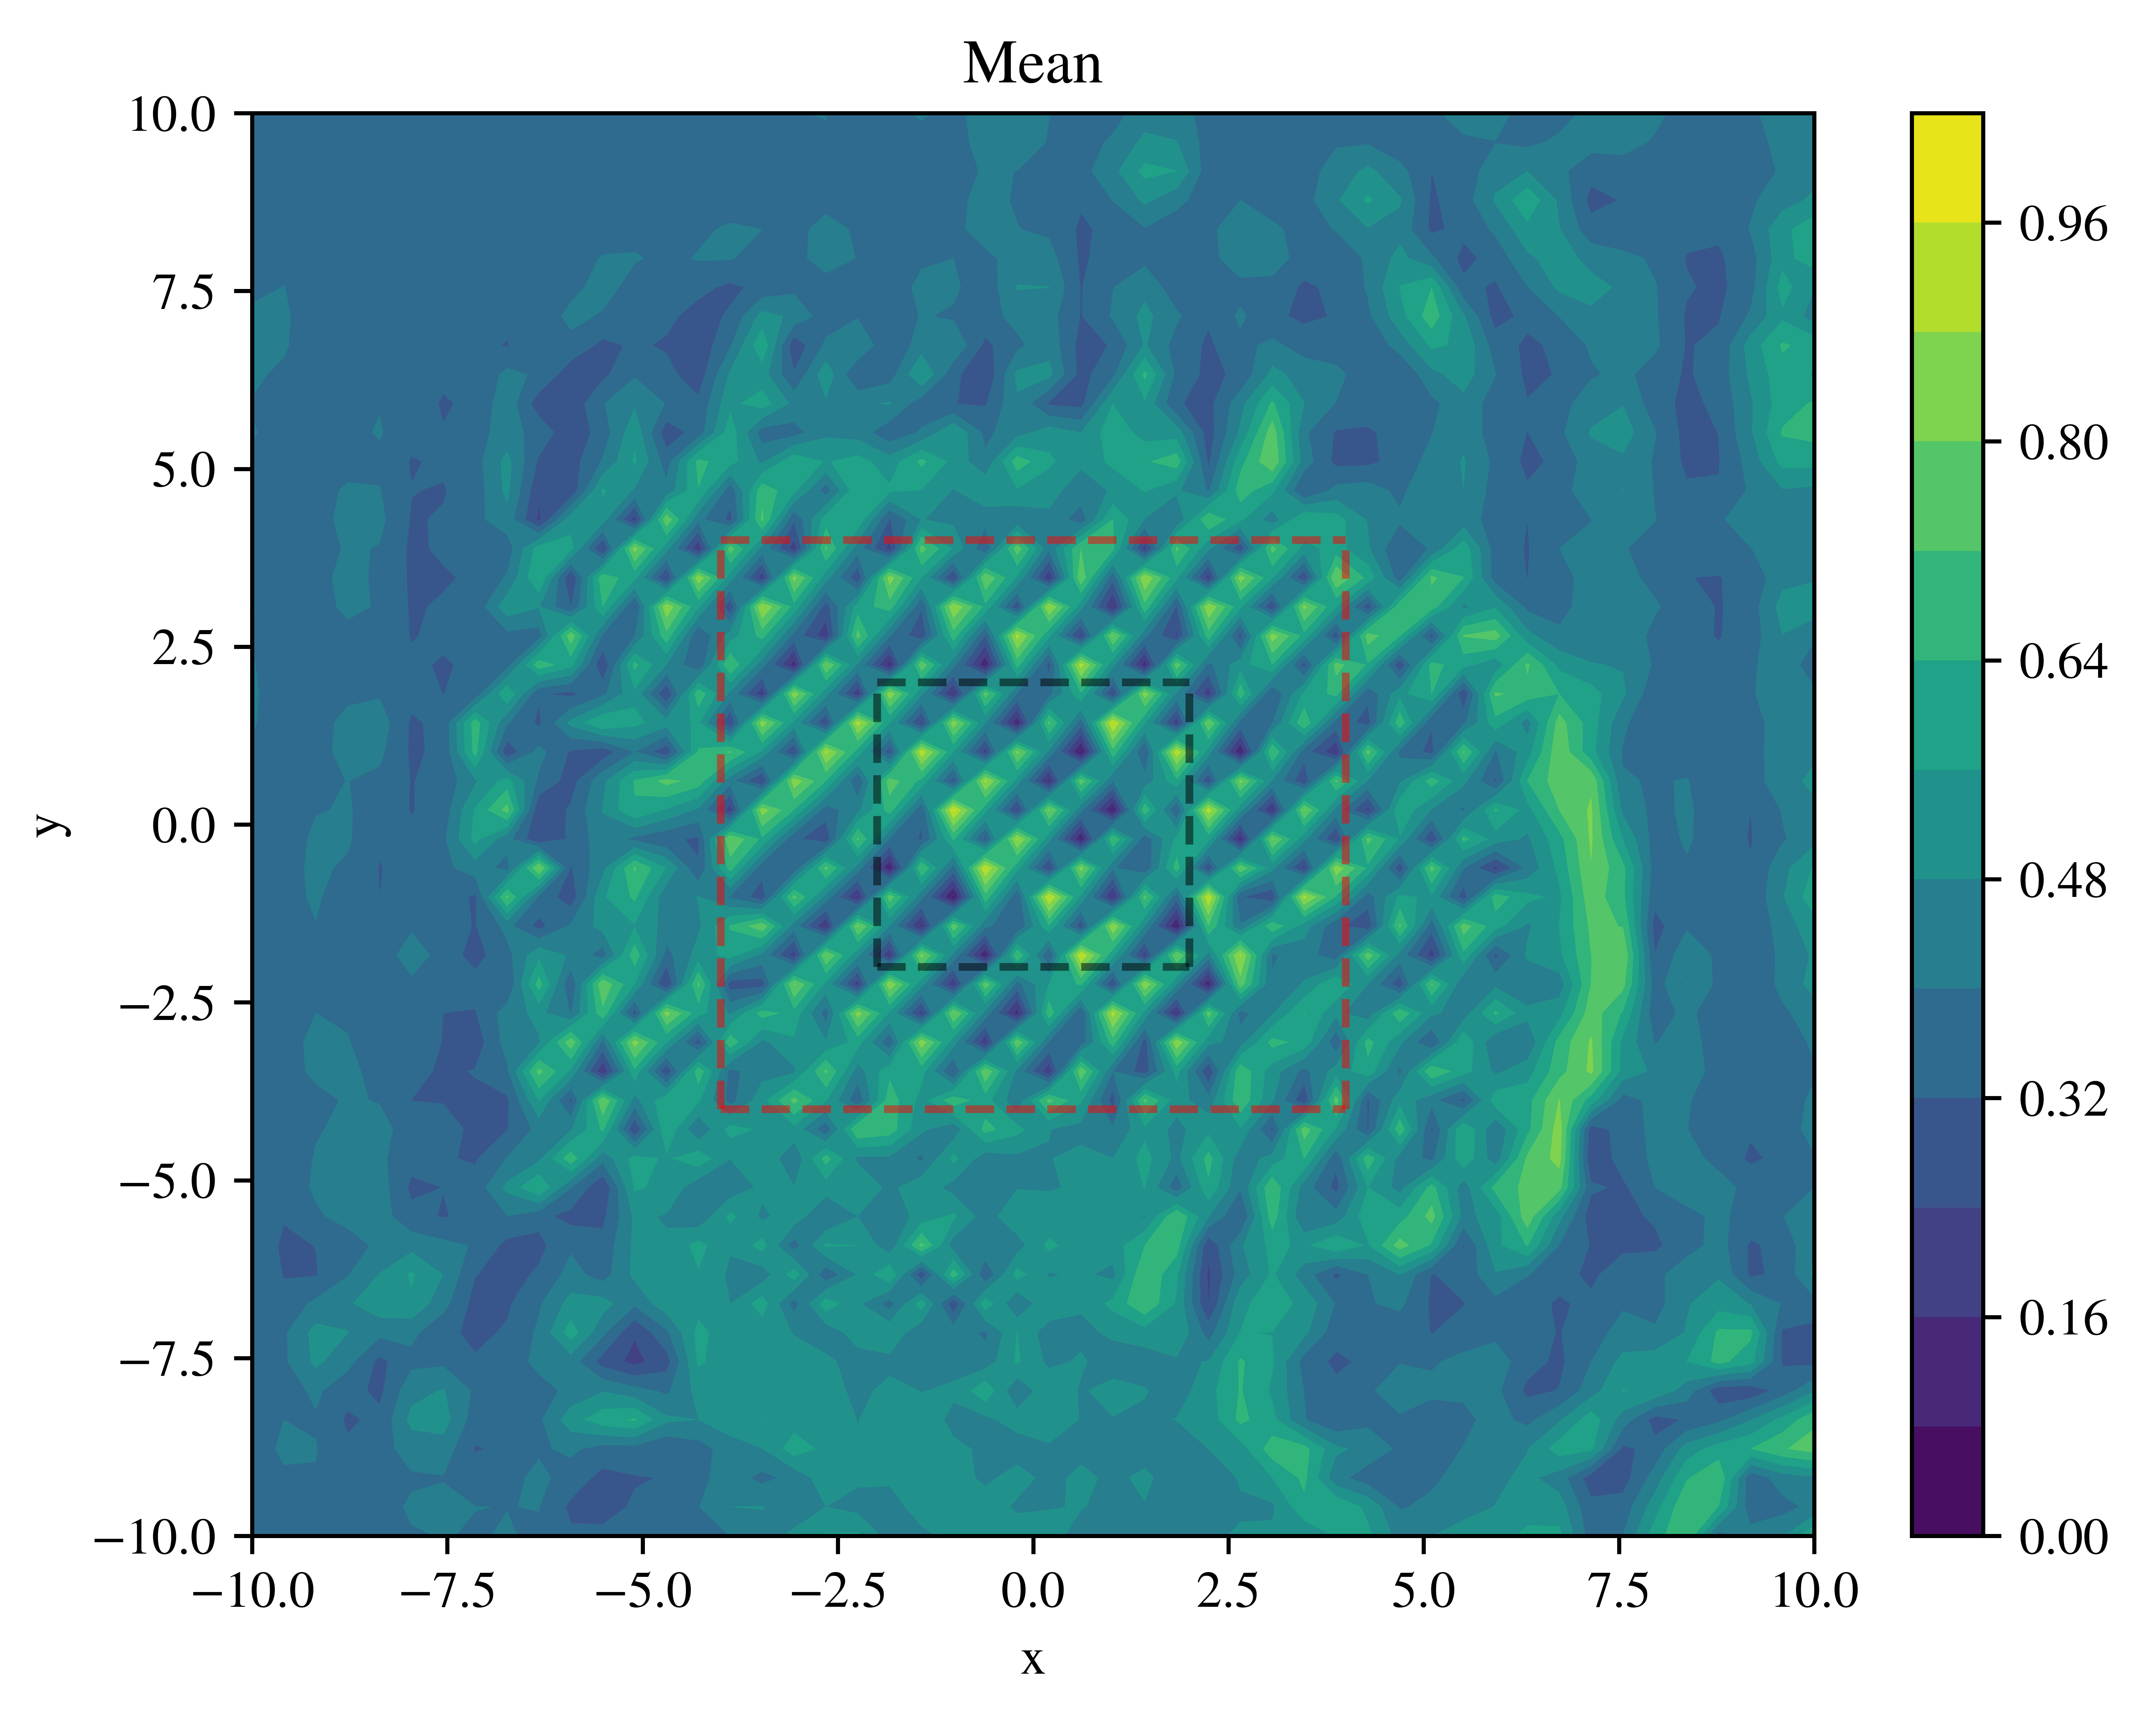
\includegraphics[width=0.3\linewidth]{./fig/conv/convnp.png}}
    \subfloat[ConvNP Sample 2]{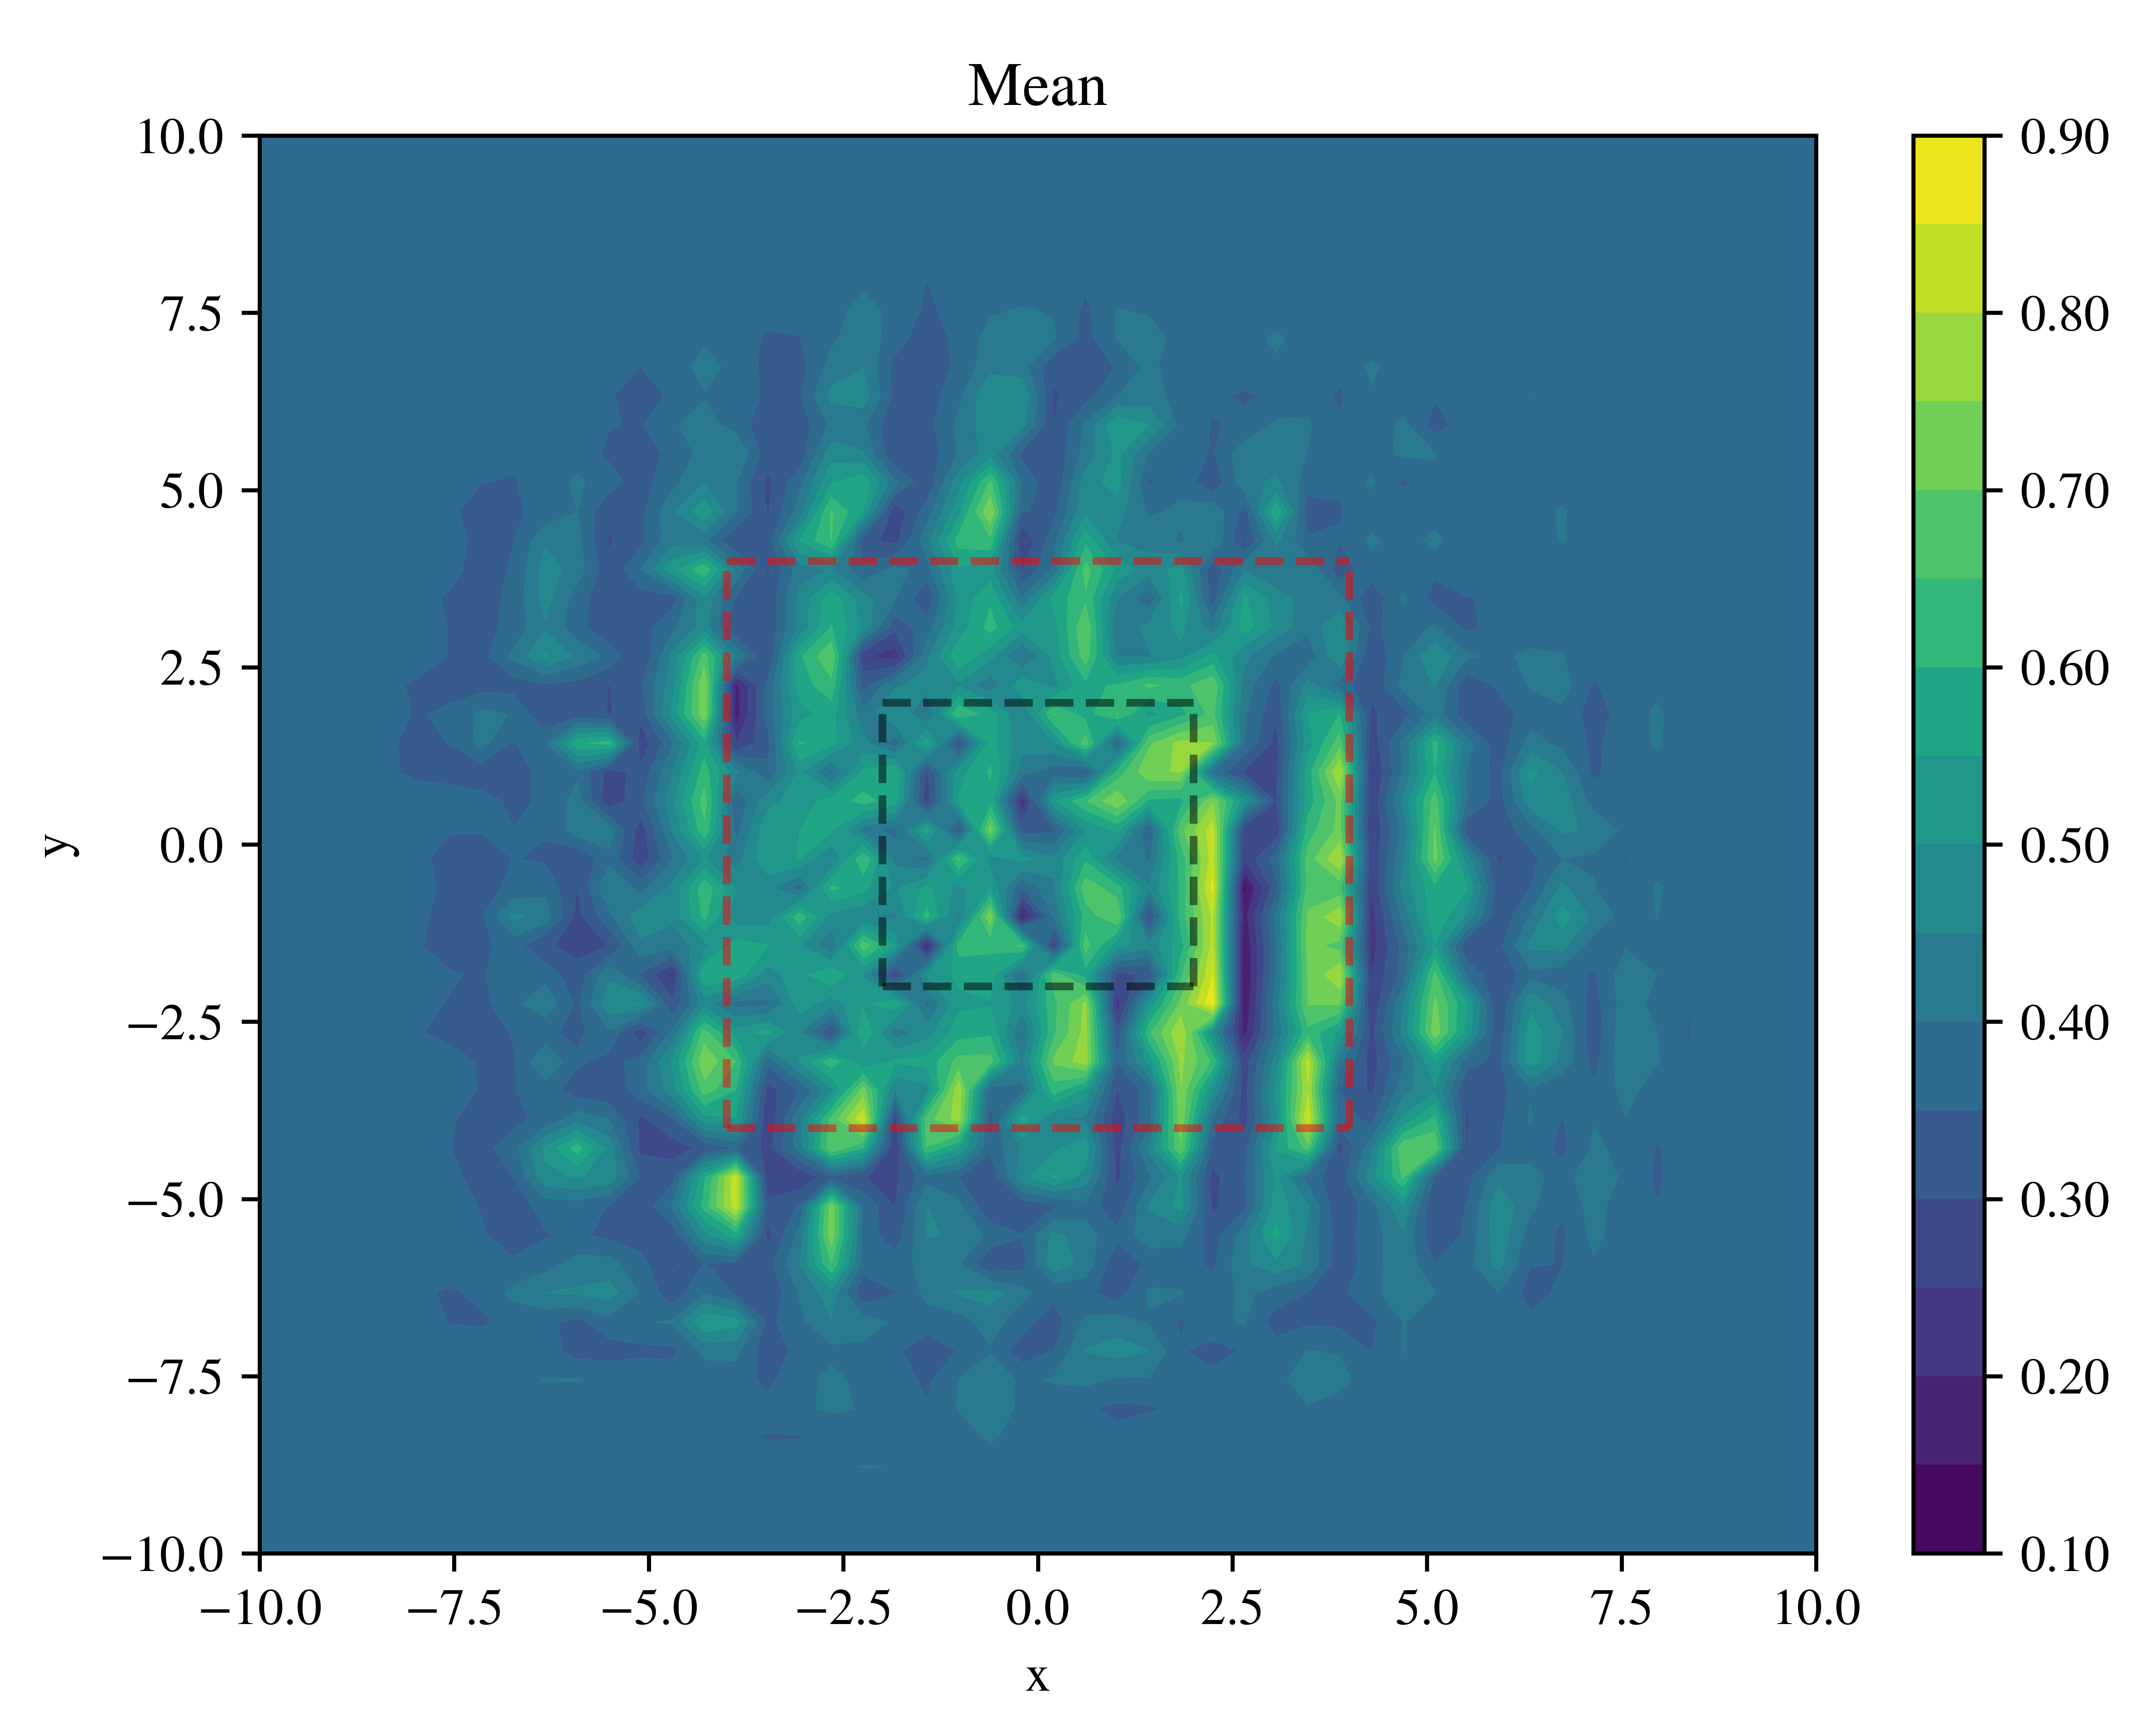
\includegraphics[width=0.3\linewidth]{./fig/conv/convnp2.png}}
    \subfloat[ConvNP Sample 3]{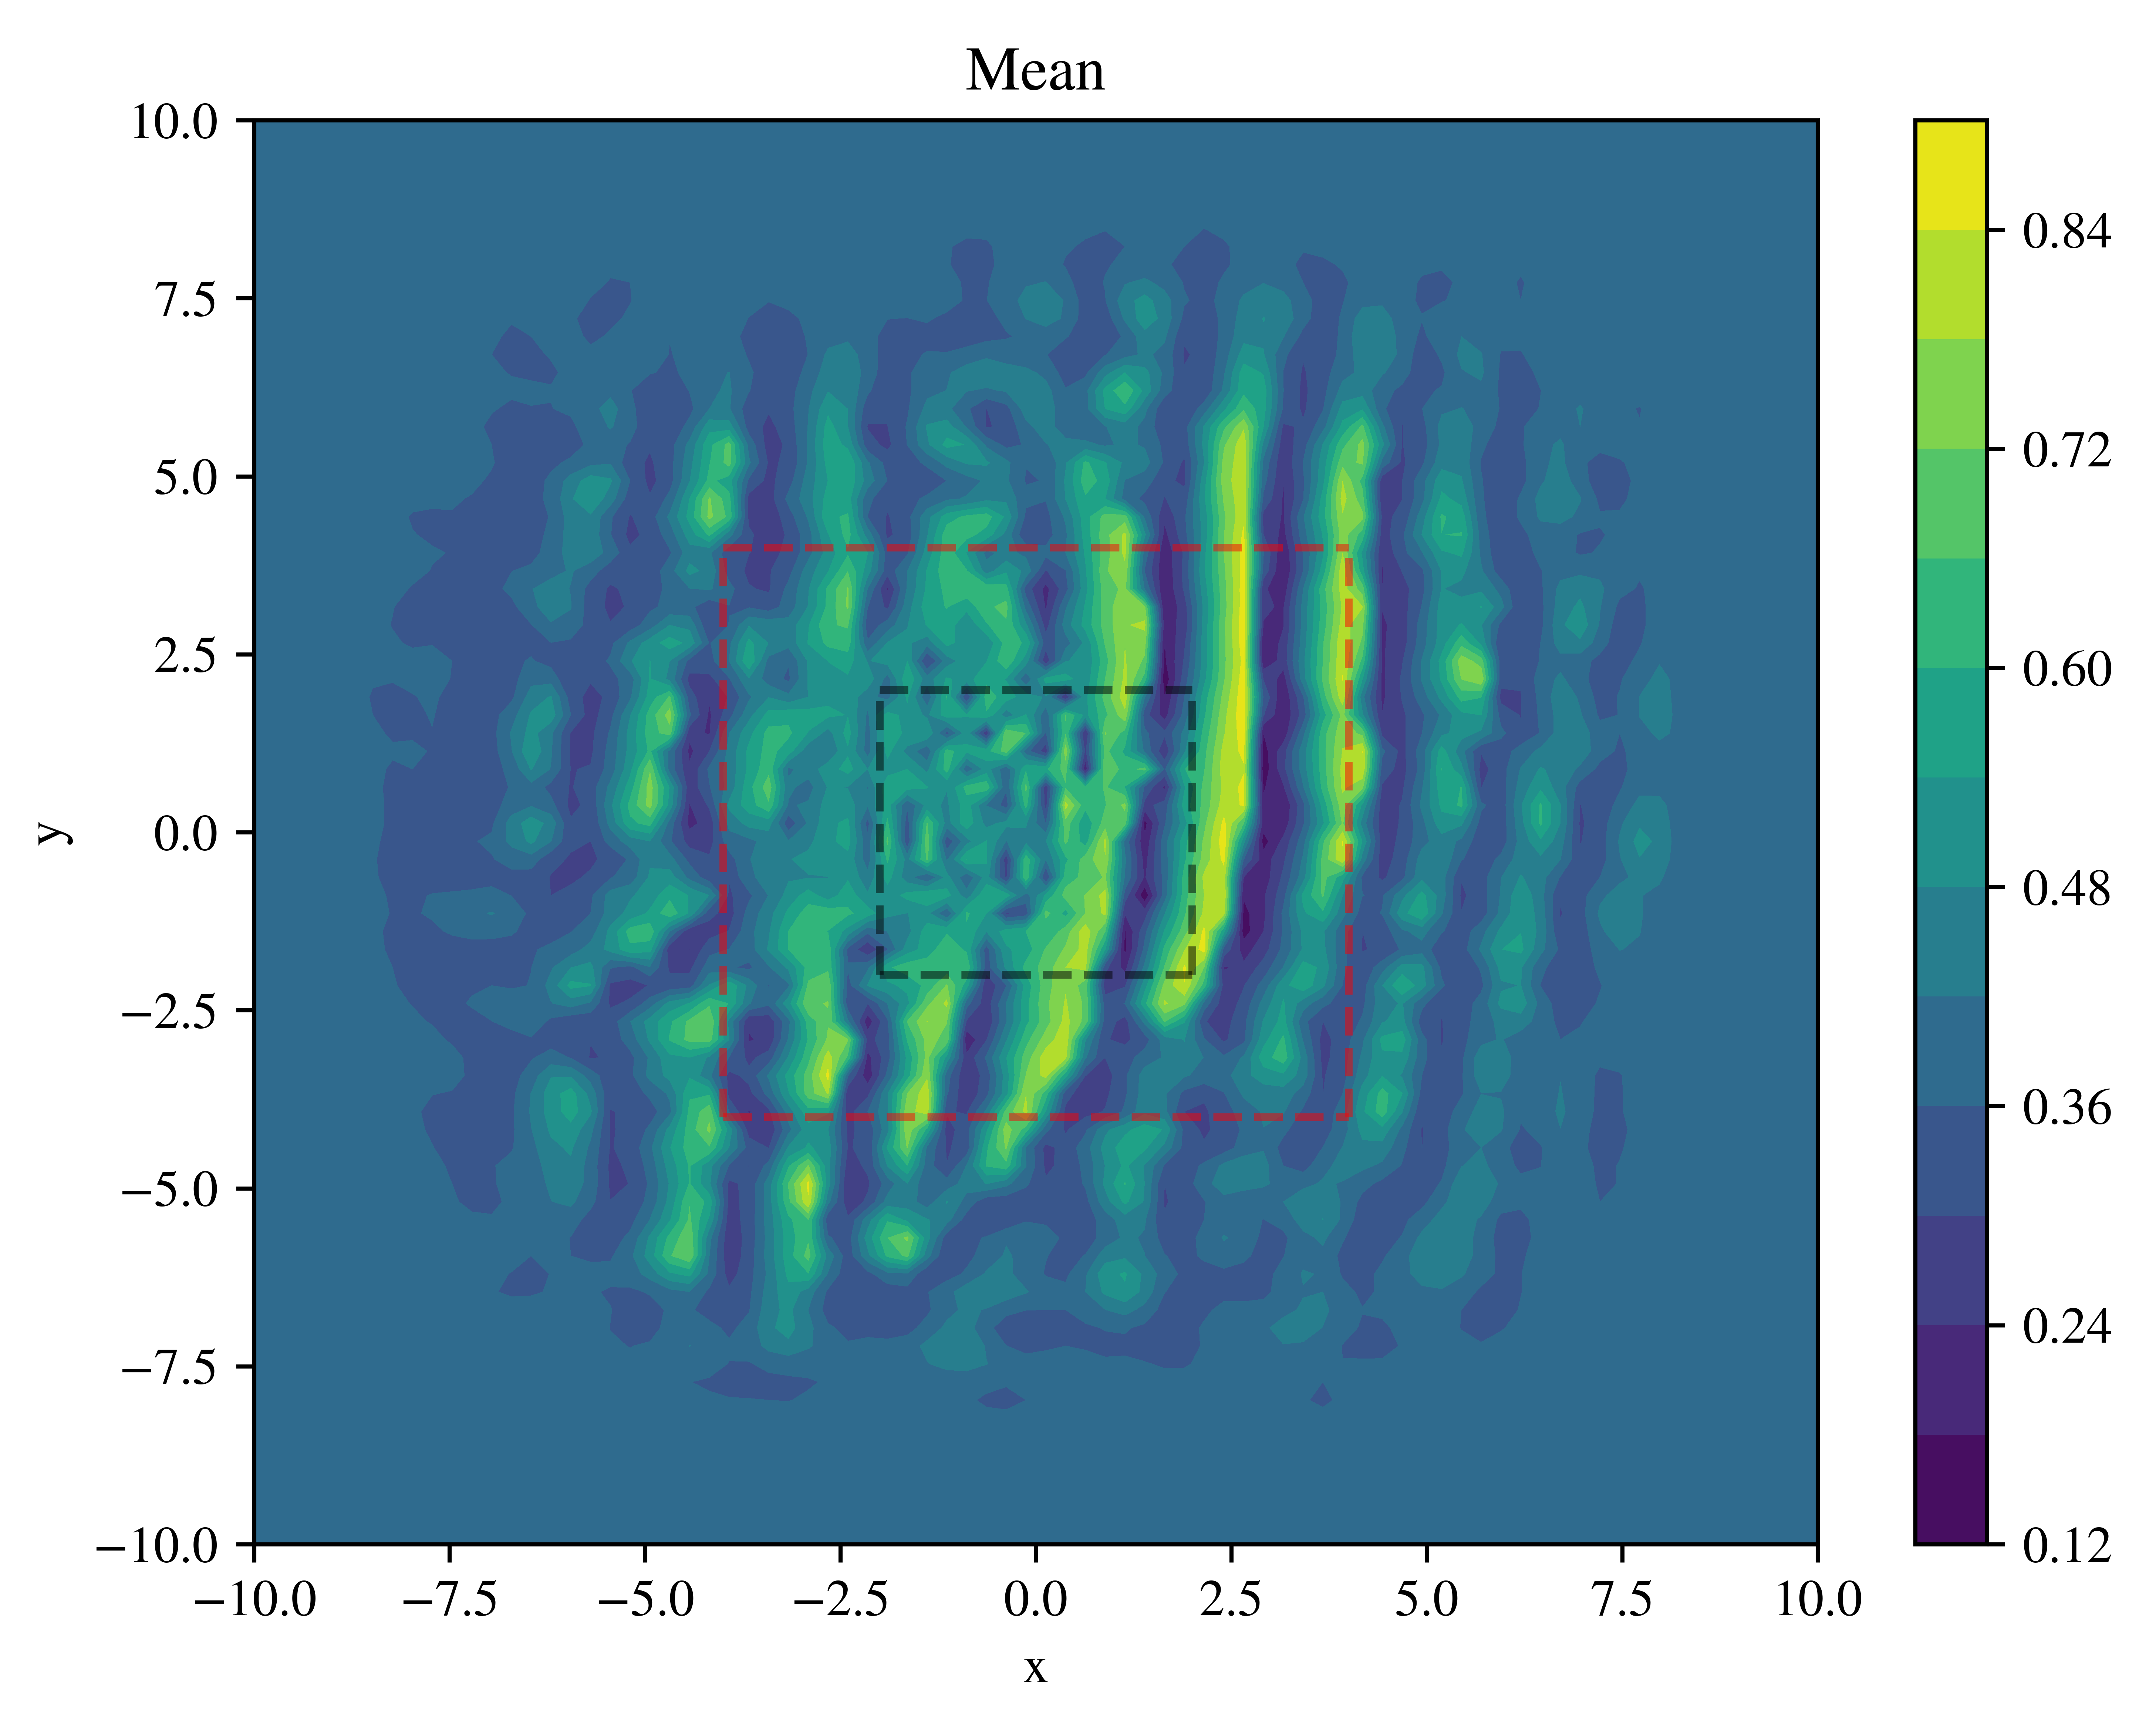
\includegraphics[width=0.3\linewidth]{./fig/conv/convnp3.png}}\\
    \caption{Samples from TETNP and ConvNP on the full Sawtooth dataset after training for 7 hours using 1 million parameters models and 64 context points. Context region is inside the black dotted box and target region inside the red dotted box. Out of the target region is the extrapolation region. Standard deviation is omitted for clarity.}
    \label{fig:full-saw-preds}
\end{figure}

The ConvNP performs terribly on the full sawtooth dataset, which may seem surprising at first, but it is not since CNNs are not rotationally equivariant. We hypothesize that the CNN will need to learn filters for the sawtooth in all directions, which is a very difficult task, especially with limited parameters. The ConvNP was able to perform well on the restricted sawtooth dataset as it only needed to learn filters for the sawtooth in \emph{two directions}. Perhaps with longer training times and more parameters, the ConvNP could learn to generalize to the full sawtooth dataset, but this was not considered in this work.

% Compared to the ConvNP the TETNP does indeed perform better in terms of validation loss.

% ./fig/conv-tetnp-saw.pdf

\begin{figure}[H]
    \centering
    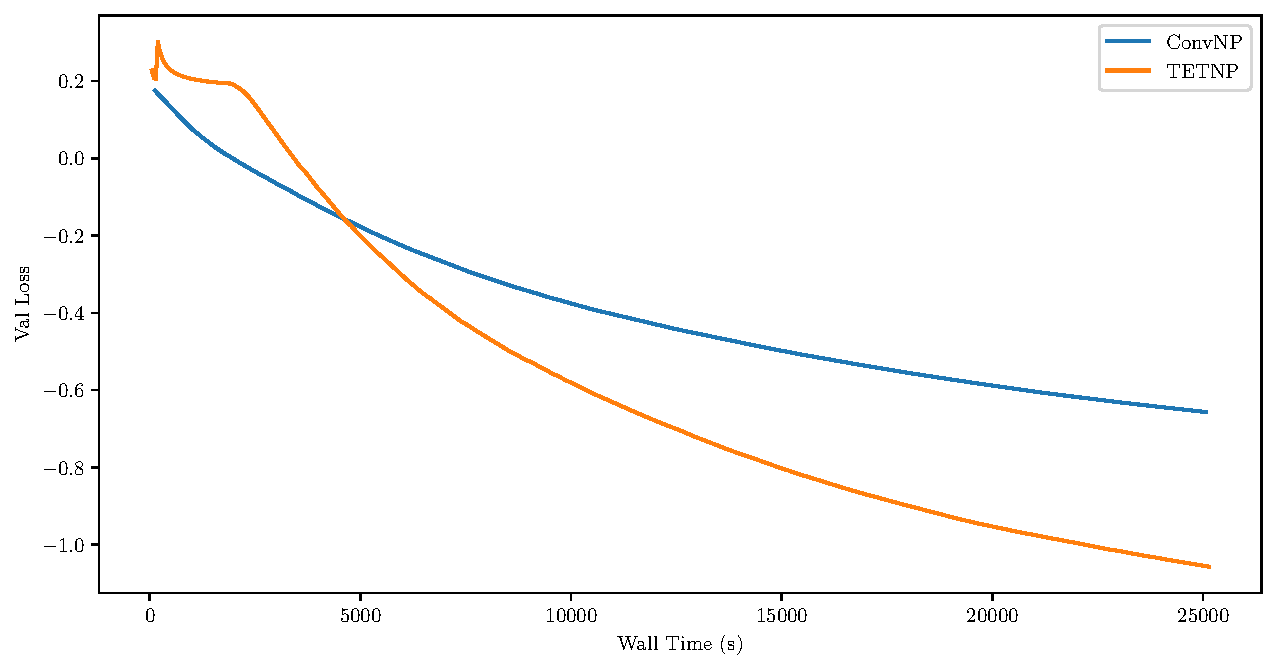
\includegraphics[width=0.6\linewidth]{./fig/conv-tetnp-saw.pdf}
    \caption{Validation Loss of ConvNP and TETNP on the 2D Sawtooth Dataset. Lower validation loss is better.}
    \label{fig:conv-tetnp-saw}
\end{figure}

\autoref{fig:conv-tetnp-saw} demonstrates that the TETNP outperforms the ConvNP by a significant margin on the full sawtooth dataset. Overall the TETNP is the clear winner and highlights the power of the Transformer architecture in learning complex patterns in the data.



\section{Computational Complexity}


\begin{table}[H]
    \centering
    \begin{tabular}{@{}llcc@{}}
    \toprule
    $N_c$ & $N_t$ & ConvNP Memory (MB) & TETNP Memory (MB) \\ \midrule
    10    & 10    & 24                 & 13                \\
    100   & 10    & 29                 & 23                \\
    1000  & 10    & 257                & 984               \\
    5000  & 10    & 1273               & 24082             \\ \midrule
    10    & 1000  & 224                & 26                \\
    100   & 1000  & 268                & 113               \\
    1000  & 1000  & 378                & 985               \\
    5000  & 1000  & 1273               & 24083             \\ \bottomrule
    \end{tabular}
    \caption{Memory usage of ConvNP and TETNP on a 2D dataset with 1 million parameter models. $N_c$ is the number of context points and $N_t$ is the number of target points.}
    \label{tab:memory-usage-comparison-2D}
    \end{table}
\FloatBarrier

\autoref{tab:memory-usage-comparison-2D} clearly demonstrates that the ConvNPs memory requirement has increased by a factor of $2^3$ compared to the 1D case \autoref{tab:memory-usage-comparison}, which agrees with the theoretical complexity of the ConvNP. On the other hand, the TETNP retains the same memory requirements as the 1D case, although it remains higher than the ConvNP. When scaling systems to higher dimensions (3D, 4D, etc.), the TETNP will be more memory-efficient than the ConvNP and will likely be the preferred choice.

\section{Summary}

In this chapter, we extended the 1D experiments to 2D and observed the performance of the ConvNP and TETNP on the Gaussian Process and Sawtooth datasets. We discovered that the TETNP outperforms the ConvNP on both datasets, with the ConvNP struggling to generalize to the full sawtooth dataset. We introduced rotational equivariance to the TETNP and observed a significant improvement in its ability to generalize to the full sawtooth dataset, when trained on the `restricted' dataset, demonstrating the ease of introducing inductive biases to the Transformer model. Finally, we compared the memory usage of the ConvNP and TETNP in 2D and observed that the TETNP scaled better than the ConvNP when increasing the number of dimensions. However, the TETNP still requires a significant amount of memory compared to the ConvNP. This motivates the need for more efficient Transformer models which will be explored in the next chapter. 


\ifSubfilesClassLoaded{%
    \printbibliography{}
}{} 


\end{document}